\part{Explorations}
\chapter{Trois Cas Observes}
\paragraph{}
Le XXIe siècle et ses innombrables moyens de communication ont rendu les
situations interculturelles de plus en plus courantes. C’est pourquoi le choc
des cultures est une expérience que chaque Français est amené à vivre
quotidiennement. Cette expérience peut émerveiller, interpeller ou choquer
comme vu ci-dessous.

\section{Emerveillement}

\subsection{1\ier version}
\paragraph{}
En France peu de tradition ont perduré au cours du temps. En effet, la France
étant un pays issue de nombreux brassage, les habitudes et les traditions sont
propres à chaque famille. Au contraire, le Japon, bien qu’étant très avancé au
niveau des nouvelles technologies, a su garder nombre de ses traditions tel que
le fait d’aller au temple prier pour la nouvelle année. Cela m’étonne toujours
avec plaisir de penser à ce contraste qui cohabite entre la culture
traditionnelle et la culture moderne japonaise.

\subsection{2\ieme version}

\paragraph{}
\begin{center}
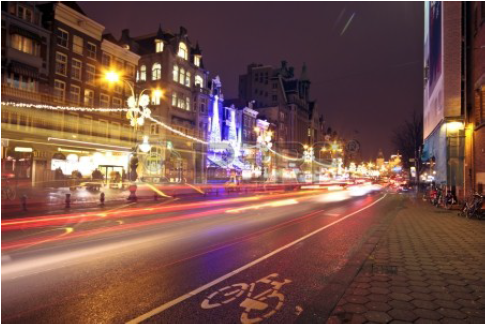
\includegraphics[scale=0.7]{Amsterdam1.jpg}
\end{center}

Parmi les situations qui m'a le plus émerveillé, c'est bien le jour où j'ai vu
deux sans abris aux alentours d'Amsterdam.  Nous étions la veille de noël et
j'ai vu ces deux personnes par terre se raconter des histoires et rigoler
ensemble. Cette scène m'a paru inespérée car il faisait froid, mais ils avaient
l'air si heureux.  Cette scène m'a fait rendre compte que nous devons profiter
de chaque moment de notre vie et que dans toutes les situations, nous devons
savoir rire et être heureux.

\paragraph{}
\begin{center}
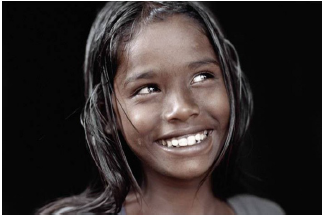
\includegraphics[scale=0.7]{Amsterdam2.jpg}
\end{center}

De nos jours, de grandes inégalités sociales ont vues le jour et nous devons
les combattre pour que personne ne meurt de froid ou de faim. Je me rends
compte que le bonheur ne vient pas seul, il faut porter de l'attention à
quiconque, car nous partageons cette même planète.  Cette expérience de vie m'a
fait comprendre beaucoup sur l'homme et sur ce dont il a besoin. Nous devons
être heureux ensemble, apprenons à vivre tous ensemble en s'entraidant.

\subsection{3\ieme version}
\paragraph{}
Des contacts interculturels qui m'ont émerveillés et qui continuent encore de
m'émerveiller sont le fait que les différences culturelles sur internet dans le
domaine de l'informatique sont complètement ignorées. En effet, lorsque le
sujet est différent de l'interculturalité les personnes sur internet parlent en
général librement sans prendre considération de l'origine ou de la culture de
l'autre. J'en conclue donc que de par le fait qu'ils n'aient pas de contacts
visuels directs avec les personnes, ils ne réfléchissent pas à l'origine ou à la
culture de l'autre, ce qui m'incline à penser que le principal facteur des
dissonances interculturelles est le contact visuel.

\subsection{4\ieme version}
\paragraph{}
Ayant peu voyagé, je n'ai pas pu connaître beaucoup de situations
interculturelles fortes. Cependant, un exemple récent me vient en tête. J'ai
suivi à la télévision et sur Internet les images des manifestations pour la
paix du 11 janvier 2015 à Paris et dans les grandes villes françaises. Alors
que le clivage entre les cultures me semblait se développer dans notre pays, et
que le « creuset français » (Gérard Noiriel) ne semblait plus une réalité,
cette manifestation m'a montré qu'une France hétérogène – dans ses origines –
mais uniforme – dans ses idéaux – existait toujours. Certes, nombreux étaient
ceux qui ont participé à ces marches pour prouver ou revendiquer une position,
comme les nombreux chefs d'État présents, ou les représentants religieux venus
dénouer les ambiguïtés entre religion et obscurantisme. Cependant, l'image
d'une foule issue de toutes les cultures et toutes les religions arborant les
couleurs françaises ou même celles de Charlie Hebdo, un journal plutôt connu
pour diviser que rassembler, était un symbole fort. Des banderoles de la
citation attribuée à Voltaire par une biographe anglaise s’étalaient en
plusieurs langues : « I disapprove of what you say, but I will defend to the
death your right to say it ». Cela peut sembler mièvre et patriotique, mais il
semblait se dégager un « esprit français ».

\begin{center}
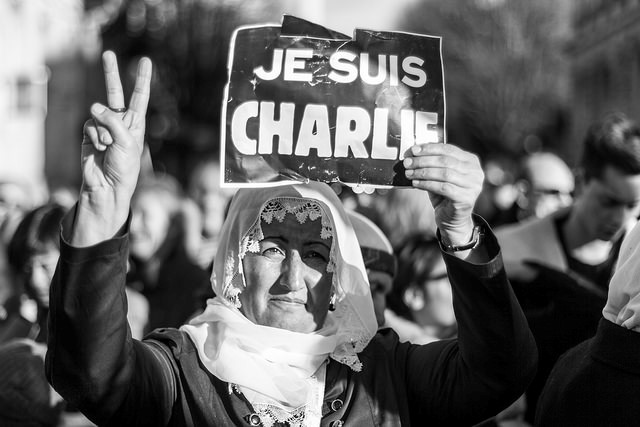
\includegraphics[scale=0.5]{charlie.jpg}
\end{center}

\section{Interpellation}
\subsection{1\ier version}
\paragraph{}
J’ai participé à trois voyages scolaires durant mes années lycée. Lors des
voyages en Irlande du Nord et en Angleterre, nous avons séjourné dans des
familles d’accueil. Lors du voyage en Angleterre, je n’ai pu apercevoir qu’une
seule fois le mari et les enfants. En effet, seule la maitresse de maison
s’occupait de nous et nous accordait du temps. Cependant, bien qu’elle fût
accueillante, nous prenions nos repas entre nous sans la famille. C’est ainsi
que nous avons passé ces quelques jours dans cette famille sans beaucoup de
contact avec celle-ci. Au contraire, lors du voyage en Irlande, nous prenions
tous nos repas avec les parents de la famille. En effet, les enfants ayant un
rythme de vie moins souple mangeaient aux heures habituelles pour leur culture
tandis que les parents nous attendaient pour manger avec nous lorsque nous
rentrions le soir. Cependant, nous avons pu voir certain des enfants le soir
qui venaient discuter avec nous et les parents pendant qu’on prenait notre
repas et eux se contentaient d’un thé. Ainsi, nous avons pu discuter des
différences de culture entre les Irlandais et les étudiants qu’ils
accueillaient, de leur histoire (ce pourquoi nous faisions ce voyage scolaire),
… Je fus donc interpellé par la différence d’accueil entre les Anglais et les
Irlandais. Bien que chacune des familles étaient payée par une association pour
nous accueillir, le ressenti ne fut pas le même : les Irlandais nous
accueillait aussi par envie et pas seulement pour l’argent.

\subsection{2\ieme version}
\paragraph{}
\begin{center}
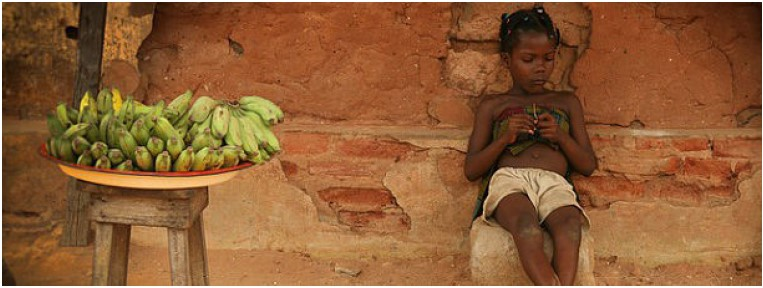
\includegraphics[scale=0.7]{Afrique.jpg}
\end{center}
Ce qui m'a émerveillé, c'est de voir ma cousine partir en Afrique, plus
précisément au Liberia, pour combattre une maladie qui a fait énormément de
mort, appelé Ébola.  Travaillant dans l'humanitaire, elle m'a toujours
passionné par tout ce qu'elle a accomplie jusqu'à présent. Ces derniers temps,
j'ai été fasciné par son courage d'entreprendre les choses et son désir de
vouloir aider ces personnes, souffrant de l’Ébola.

\paragraph{}
\begin{center}
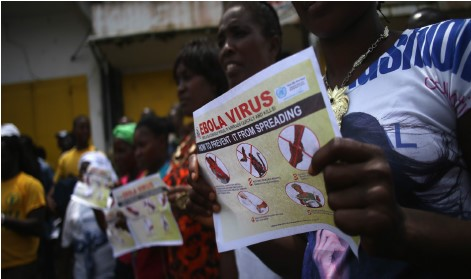
\includegraphics[scale=0.7]{Afrique2.jpg}
\end{center}
Actuellement, elle est une des managers d'une ONG en santé publique, permettant
de limiter la contamination du virus. Elle me raconte par mails ses journées et
comment est-ce qu'elle fait pour ne pas craquer émotionnellement. Ses
différentes expériences à travers le monde m'ont donné l'envie de voyager et
d'aider les personnes qui m'entourent.

\subsection{3\ieme version}
\paragraph{}
Ce qui m'a interpellé lors d'un voyage en Allemagne est le fait que les
allemands mangent de la charcuterie au petit déjeuner. Après des études
approfondies, j'ai jugé que ce rituel culturel méritait sa place en Allemagne
et sûrement dans d'autres pays. C'est du moins ce que mes papilles gustatives
en ont déduit.

\subsection{4\ieme version}
\paragraph{}
Il y a près de quatre ans, je suis parti en Angleterre pendant deux semaines
avec un ami. Ses parents l’avaient poussé à partir pour un séjour linguistique
en groupe, et je l’ai accompagné. Je me suis donc retrouvé avec lui en famille
d’accueil, et je pensais que nous serions souvent en contact avec les « natifs
». J’ai assez vite déchanté : les familles d’accueil sont une industrie
anglaise ! Dans cette petite maison, nous étions quatre étrangers d’origines
différentes, mais la famille habituée ne jouait pas la carte du melting-pot :
nous étions dans des chambres différentes, nous n’étions pas soumis aux mêmes
horaires, nous avions rempli un formulaire sur les plats que nous n’aimions
pas… De même, lors des sorties organisées par le groupe, et lors des cours
d’anglais organisés par un professeur non francophone, les jeunes français (qui
pourtant ne se connaissaient pas) s’isolaient pour discuter entre eux. Cela
peut sembler naturel : timidité, hésitation à parler en anglais… Mais les
organisateurs ne faisaient rien contre, que ce soient les Français tout aussi
hésitants ou les Anglais habitués à ce genre de situation. Finalement, je n’ai
pas progressé en anglais au cours de ce voyage, et n’ai connu aucune situation
interculturelle. Bien que timide de nature, j’en étais très déçu.


\section{Choc}
\subsection{1\ier version}
\paragraph{}
Un été je suis partie une semaine en Toscane. Ne pouvant pas marcher longtemps
suite à de nombreuses entorses, nous avons fait le tour de la Toscane en
voiture en nous arrêtant dans les villes plus ou moins touristique sur notre
chemin (Florence, Pise, …).  En arrivant sur Florence, nous avons pris une
route à deux voies. Nous avons vu devant nous trois voitures côtes à côtes.
Cela m’a choqué de voir ce manque de respect pour le code de la route et ce
mépris du danger. En effet, les Français ne sont pas toujours les meilleurs
dans le respect du code de la route mais ça n’en devient pas un sport national
comme en Italie : nous avons vu de nombreuses absences de respect du code de la
route.

\subsection{2\ieme version}
\paragraph{}
\begin{center}
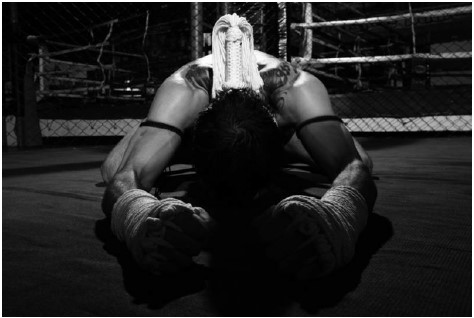
\includegraphics[scale=0.7]{Thai1.jpg}
\end{center}

Lors d'un voyage à Thaïlande, j'ai décidé de découvrir la boxe thaïlandaise,
appelé plus communément « Muay Thai » dans le pays de provenance de cet art
martial. La boxe thaïlandaise se base sur quatre techniques fondamentales :
les coups de poings, pieds, genoux et coudes. Les boxeurs portent des gants et
un short afin de faciliter les mouvements des jambes. Les combats s'effectuent
en 5 reprises de 3 minutes entrecoupées de pause de 2 minutes. Le tout se
déroule sur une musique de fond thaïlandaise très envoutante.  Quelques jours
après mon arrivée, je me baladais dans les rues du quartier de Sukhumvit, dans
des avenues très vivantes, jours et nuits sur toute leur longueur, je me suis
dirigé vers un bâtiment qui ressemblait à un temple. Tout le monde criait et
voulait y rentrer, j'ai convaincu les amis avec qui j'étais d'y aller, pour
voir de quoi est-ce qu'il s'agissait.  L'entrée était gratuite, mais il y avait
des guichets où nous pouvions miser de l'argent sur des numéros. Ces numéros
étaient tout simplement des boxeurs et nous étions arrivés en face d'un ring de
boxe autour duquel se trouvait une foule incroyable.

\begin{center}
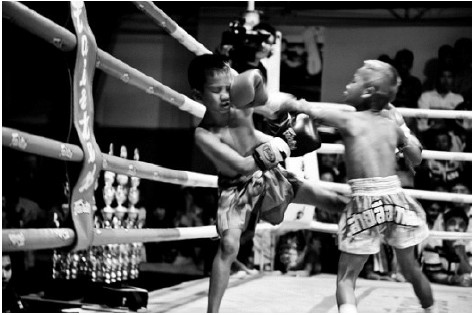
\includegraphics[scale=0.7]{Thai2.jpg}
\end{center}

\paragraph{}
Sur le ring, se trouvait deux enfants âgés de 8 ans combattant l'un contre
l'autre sous les applaudissements et les encouragements d'adultes qui criait
victoire pour la personne sur laquelle il avait misé. Cette scène eut l'effet
d'un tonnerre qui s'abattit sur moi, car je ne pouvais rien à faire pour arrêter
ce massacre.  Malheureusement, j'ai demandé aux spectateurs la raison pour
laquelle ils se battaient et on me répondit « de baht ! », qui veut dire « pour
l'argent » en thaïlandais. Totalement outragé de voir ce qu'il se passait en
Thaïlande, j'ai décidé de retrouver le jeune boxeur ayant perdu et n'ayant pas
gagné d'argent, pour le féliciter et lui donner 400 bahts, qui est l'équivalent
de 10 euros, mais qui représente une somme énorme pour eux.  Ces découvertes
m'ont mis totalement mal à l'aise et j'ai décidé de combattre cette cause en
revenant à la source, la pauvreté.

\begin{center}
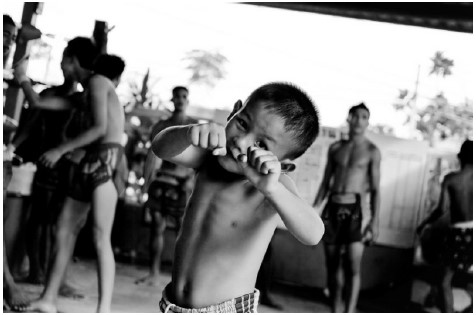
\includegraphics[scale=0.7]{Thai3.jpg}
\end{center}


\subsection{3\ieme version}
\paragraph{}
Une situation qui m'a choqué en étant en voyage au Sri-Lanka est la conduite de
ces derniers. En effet, il m'est arrivé d'être à quatre voitures sur une route
à deux voies à sens alternés. J'en ai donc déduit que les Sri-Lankais se
faisaient confiance au point d'avoir ce genre d' « interactions » sur la route.

\subsection{4\ieme version}
\paragraph{}
Ma famille est très attachée au patrimoine : mon père et ma mère sont des
spécialistes des monuments historiques, mon grand-père et mon oncle sont
antiquaires. J’ai donc été élevé dans cette ambiance, ne partant en voyage que
pour visiter des églises. C’est pourquoi, lors d’un séjour à Venise où, étant
très jeune, je ne prêtais pas grande attention à la culture locale, j’ai été
frappé par l’approche différente que l’Italie a de la culture. En effet, de
nombreuses églises, du fait du nombre de touristes, font payer les visiteurs à
l’entrée ! Cela me semblait inconcevable, d’autant que je n’étais pas certain
que cet argent irait à la paroisse ! Plus tard, lors d’un voyage scolaire à
Pompéi, j’ai remarqué l’état de délabrement de la cité millénaire, qui est dû à
l’absence de moyens de conservation plus qu’aux dégâts infligés par le Vésuve.
Plusieurs bâtisses se sont effondrées, redressées à la va-vite avec du béton et
cachées à la vue des visiteurs par des pancartes. Un bâtiment du forum a même
été transformé en cafétéria. Ma mère m’expliqua que l’argent des visiteurs
n’allait pas à la conservation du site mais plus ou moins à la pègre locale
(n’oublions pas qu’il s’agit de Naples !). Si l’Italie comme la France jouit
d’un patrimoine exceptionnel, l’approche italienne est beaucoup plus économique
! J’en étais d’autant plus attristé qu’avec Pompéi peut disparaître une portion
d’histoire.

\begin{center}
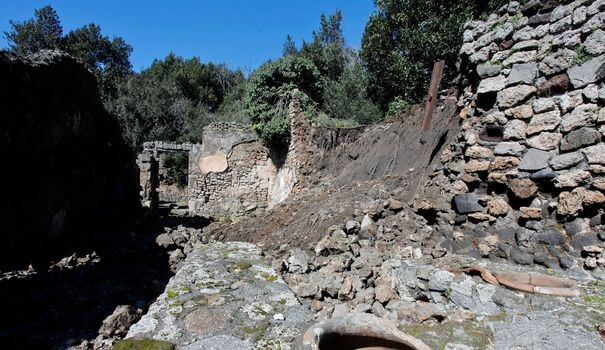
\includegraphics[scale=0.5]{Pompei.jpg}
\end{center}


\chapter{Bienvenue au café}
\paragraph{}
Chaque café possède sa propre vie, sa propre ambiance qui varie suivant
l’heure, le jour et leur voisinage. Du café de la gare peuplé de voyageurs au
comptoir montagnard abritant les skieurs frigorifiés, en faisant un détour par
Londres, nous allons vous donner un aperçu de l’atmosphère typique de ces lieux
de rencontres.

\subsection{1\ier version}
\paragraph{}
La vie des cafés varie grandement suivant leur situation géographique, la météo
et la période.

\paragraph{}
Prenons deux cafés dans une même station de ski familiale dans le massif
central : la brasserie des pistes, vu entre 18h45 et 19h30, fait
bar/brasserie/restaurant ; le polar beer, vu entre 16h et 17h, fait bar toute
la journée et snack le midi. Il se situe juste en bas des pistes.

\begin{center}
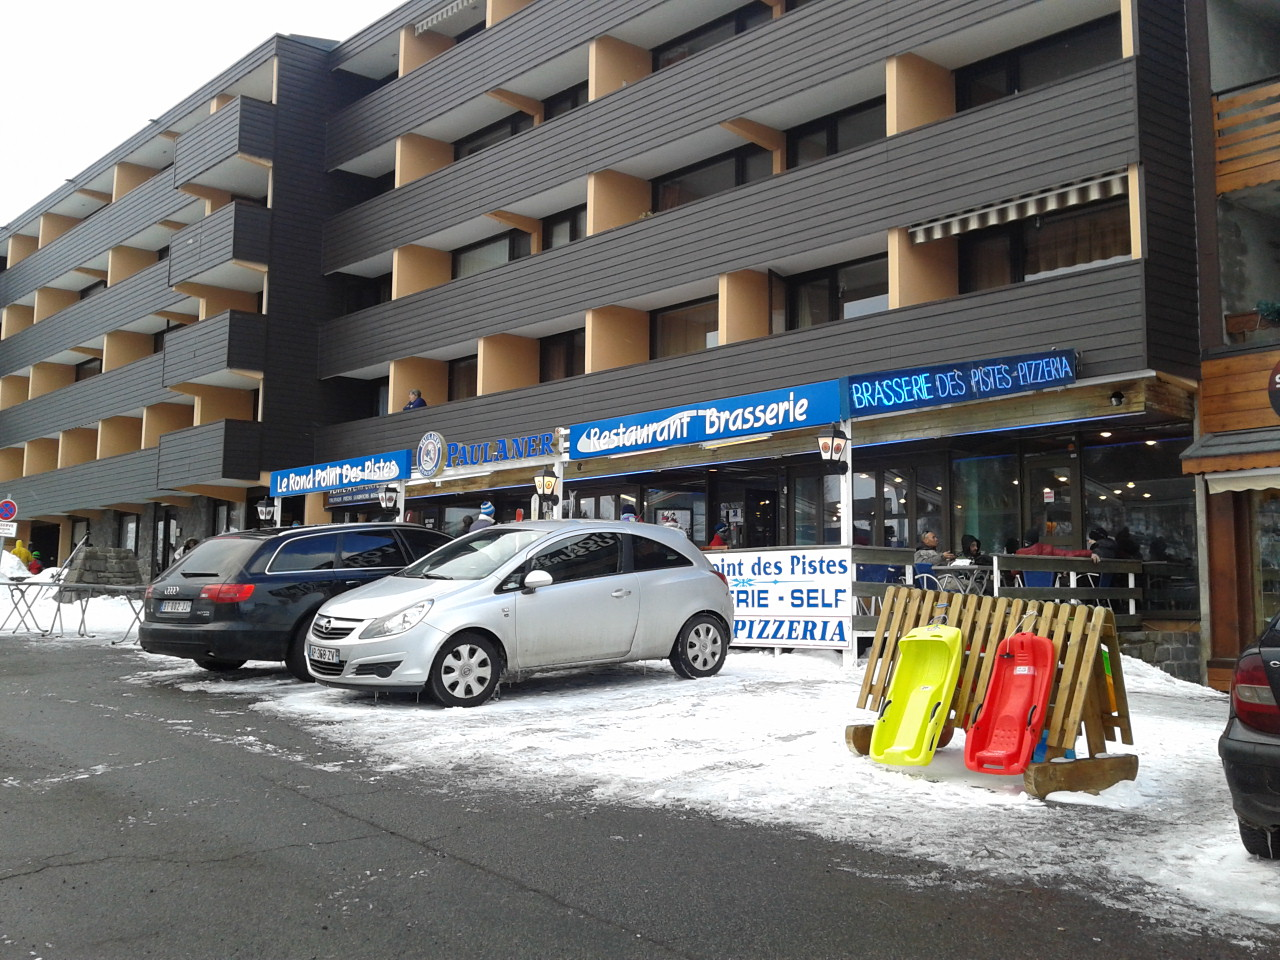
\includegraphics[scale=0.15]{brasserieDesPistes.jpg}
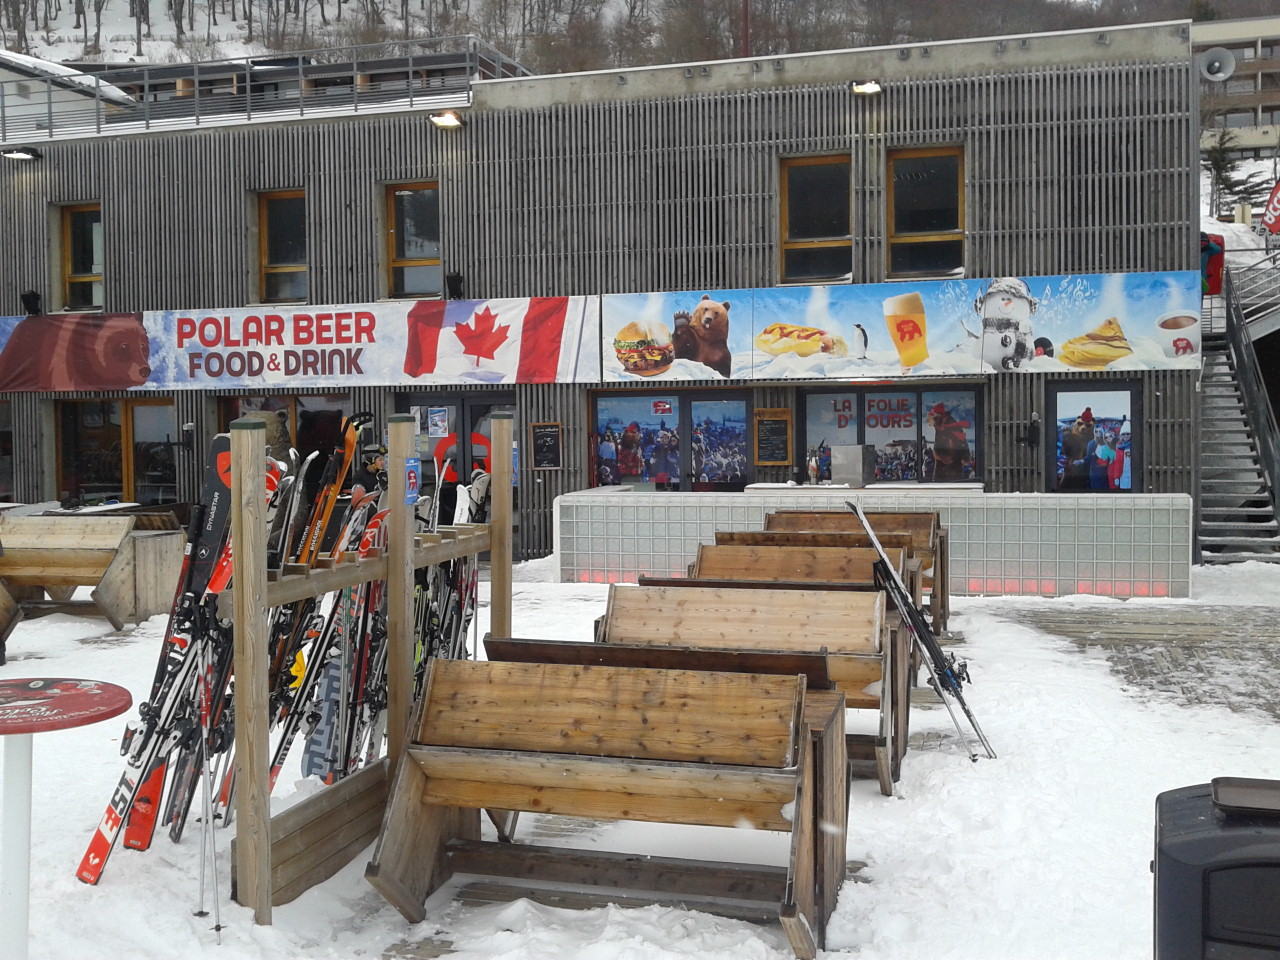
\includegraphics[scale=0.15]{PolarBeer.jpg}
\end{center}

\paragraph{}
À la brasserie des pistes, il y avait le patron, la patronne au bar, le
cuistot, le pizzaiolo, et deux serveurs. Au contraire, au polar beer, il n’y
avait que deux serveuses. Cette différence s’explique par le fonctionnement de
chacun des établissements. En effet, étant servi à table à la brasserie des
pistes, il est nécessaire d’avoir plus de personnel qu’au polar beer où les
clients doivent aller chercher leurs consommations au comptoir. De plus, dans
chaque café la consommation est payée au moment de la prise en main de
celle-ci.

\paragraph{}
Dans chacun des établissements il y avait une télévision. A la brasserie des
pistes, la télévision permet d’écouter RFM TV sauf au moment du journal
télévisé régional où l’on bascule sur France 3. Au contraire, au polar beer, la
télévision montrait des surfeurs et il y avait de la musique lounge en fond
sonore. On pouvait cependant remarquer que c’était surtout les adolescents et
jeunes adultes masculins qui regarder la télévision au polar beer quand
personnes ne regardait la télévision à la brasserie des pistes.

\paragraph{}
La décoration de la brasserie des pistes était basique : des tables carrées
pour la partie restaurant et quelques tables rondes pour la partie bar, des
chaises en fer, quelques banquettes. Au contraire, au polar beer, la décoration
était moderne et humoristique : des tables hautes, longues ou rondes avec des
chaises hautes, les murs étaient principalement rouges avec des jeux de mots
par-ci, par là tels que « beer crossing » d’un côté du mur et « bear crossing »
de l’autre. De plus, le comptoir était séparé en deux parties distinctes : le
bar où des bouteilles étaient exposées juste derrière et une partie snack
servant uniquement les boissons chaudes, crêpes et gâteaux à cette heure-ci.

\begin{center}
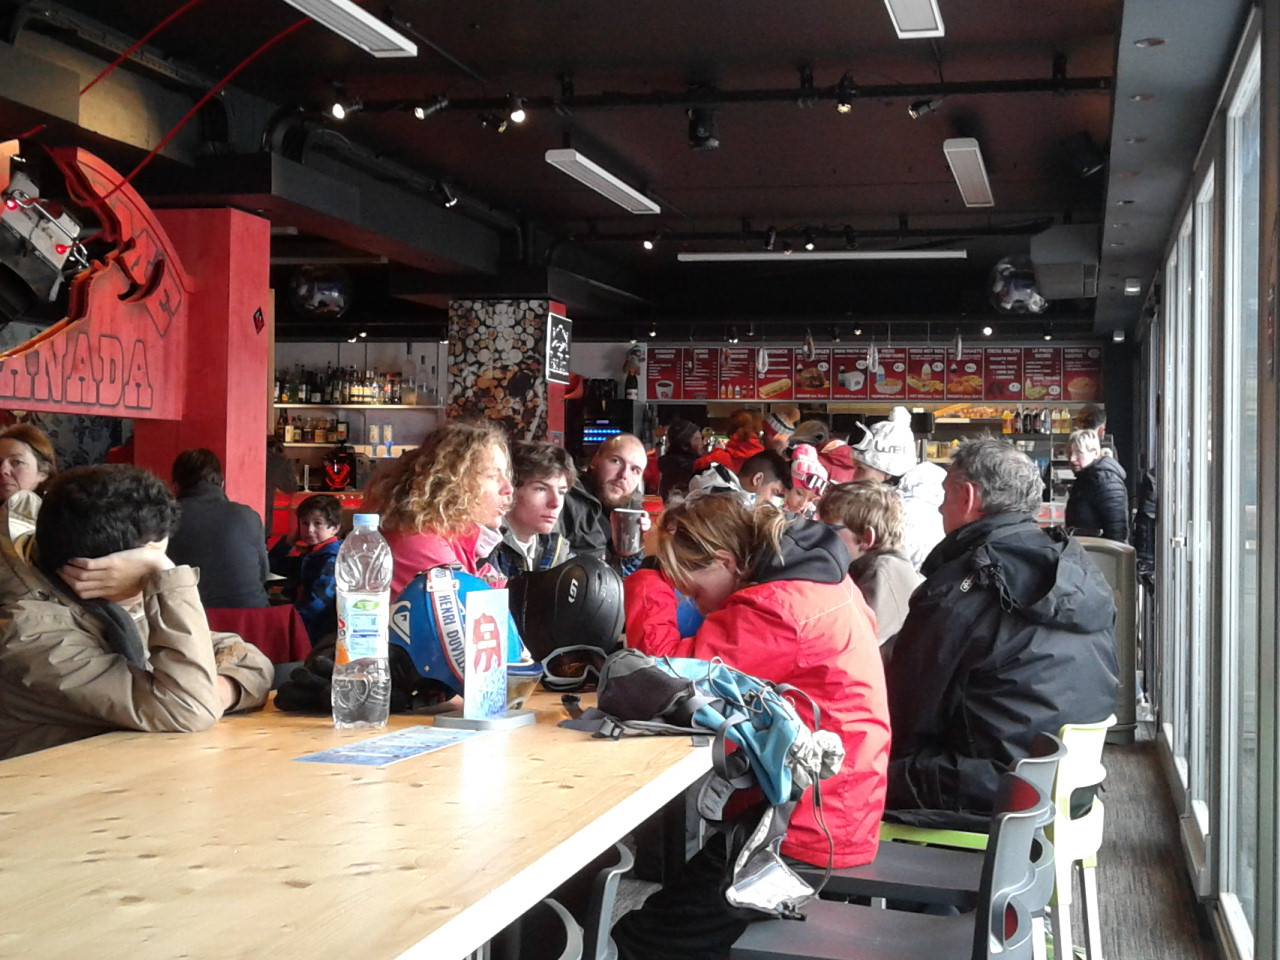
\includegraphics[scale=0.15]{PolarComptoir.jpg}
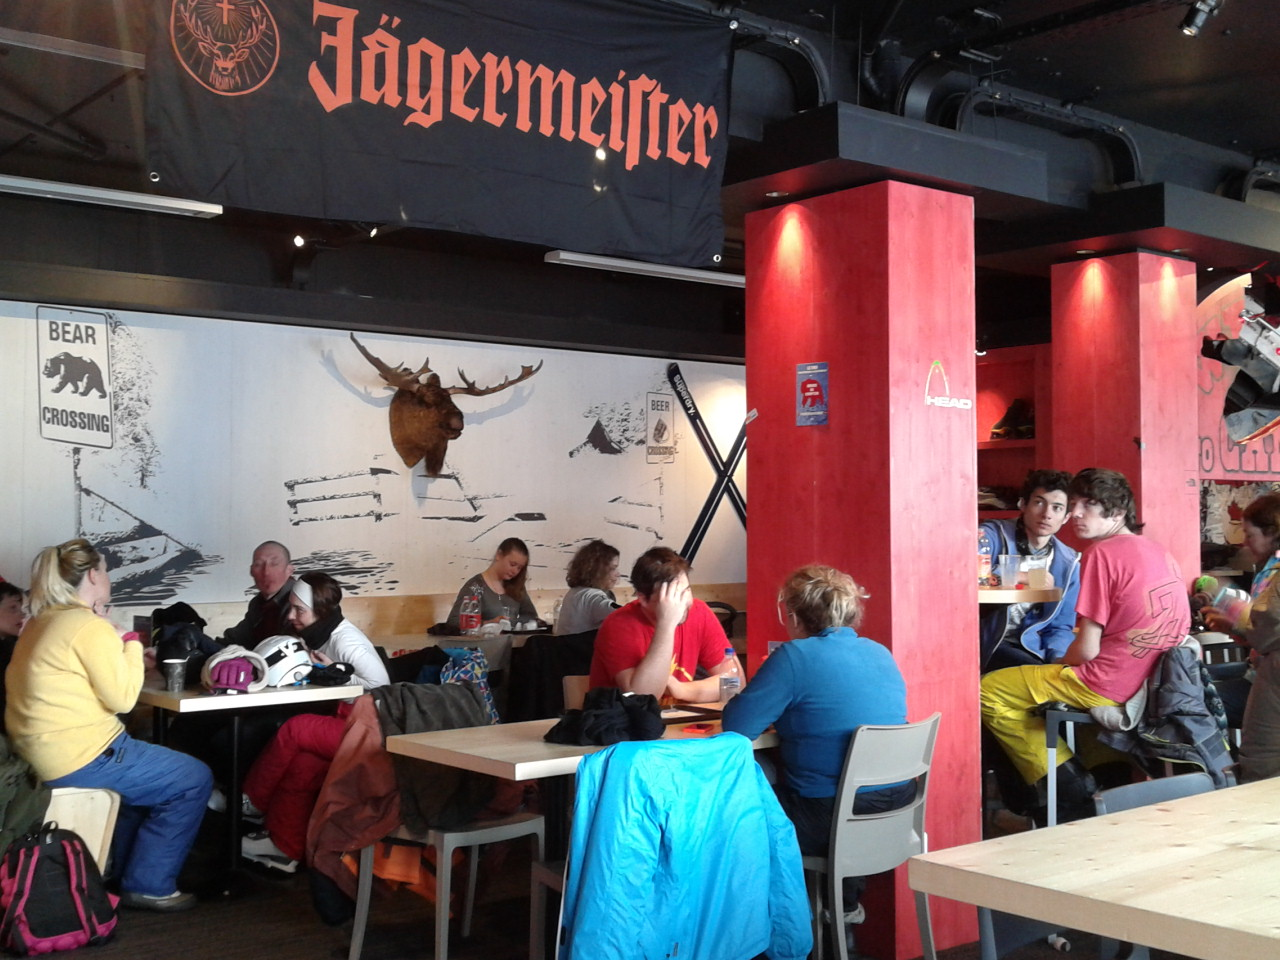
\includegraphics[scale=0.15]{PolarDeco.jpg}
\end{center}

\paragraph{}
La population de chaque café était également différente.

\paragraph{}
En effet, à la brasserie des pistes, il n’y avait personnes entre 18h45 et
19h00. Puis deux types de personnes sont arrivés peu à peu : il y avait les
familles avec enfants qui venaient diner et deux duos qui venaient boire un
coup. L’un des duos était des hommes d’environ trente ans qui ont pris chacun
deux vins chauds en jouant aux cartes. Le deuxième duo était un couple ayant
environ la soixantaine qui a également pris un vin chaud par personne. Ce choix
de boisson s’explique par la situation géographique du café : c’est une boisson
qu’on boit souvent au ski. Vers 19h30, la plupart des tables du restaurant
étaient prises par les familles avec enfants voulant diner. De plus, j’ai pu
remarquer que le comportement des serveurs variait avec les enfants : ils
prenaient un ton paternaliste et était aux petits soins. Enfin comme il
pleuvait et neigeait, la terrasse était vide.

\paragraph{}
Au polar beer, la population était constituée de skieurs. Vers 16h, il
s’agissait principalement de famille tandis que vers 16h45, la population
arrivante était principalement des groupes de jeunes adultes. Certains
restaient avec leur manteau et repartait après avoir bu leur consommation et
s’être un peu réchauffé. D’autres se déshabillaient un peu plus et restaient
plus longtemps. La principale consommation était des chocolats chauds même si
certains adolescents buvaient des sodas.  Certains sodas et la bière étaient
d’origine locale tel que l’ « auvergnat cola ». Enfin, le soleil étant au
rendez-vous bien qu’un peu couvert, les fumeurs consommaient leurs boissons et
crêpes sur la terrasse tout en fumant.

\begin{center}
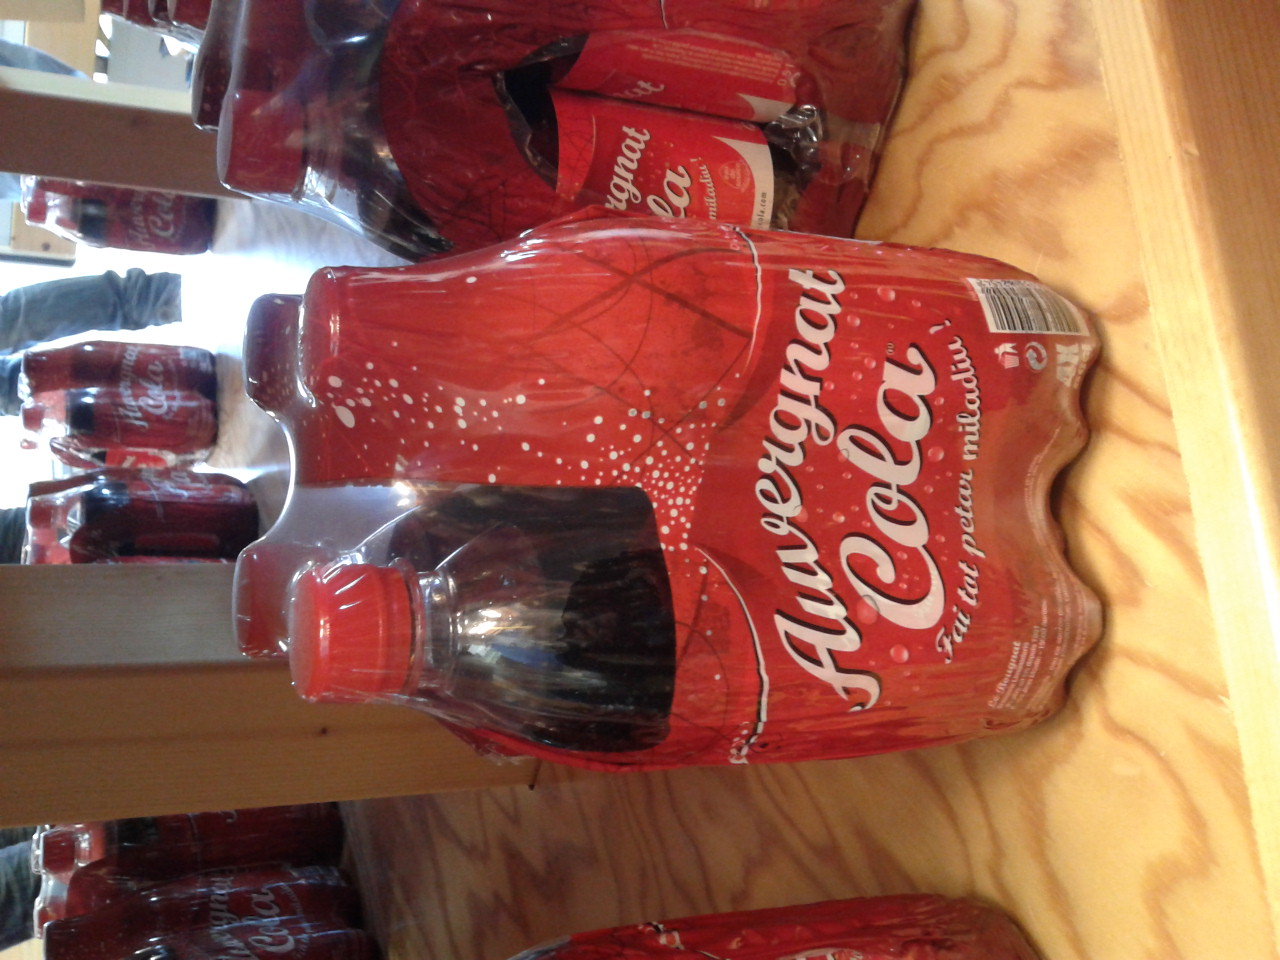
\includegraphics[scale=0.15,angle=270]{AuvergnatCola.jpg}
\end{center}

\paragraph{}
De plus, si on compare la vie de ces deux cafés à celle d’un café de campagne,
on se rend compte que c’est encore différent.

\paragraph{}
En effet, le vendredi, jour de marché, de 11h à 11h30 en août à Arcis sur Aube,
petite ville de 3000 habitants, le café et sa terrasse sont bondés. Cette
densité de population au sein de café est due au fait que les habitués s’y
retrouvent pour discuter des dernières nouvelles. Mon grand-père étant un
habitué, il s’arrête à chaque table pour dire bonjour aux gens qu’il connait.
Puis il entre dans le café et dire bonjour au patron tout en commandant un
café. Ensuite, il va s’assoir avec une de ces connaissances, en l’occurrence
une grand-mère et ces trois petits enfants. La serveuse apporte le café. Les
petits enfants jouent au babyfoot pendant que les grands-parents discutent des
dernières nouvelles. Les personnes travaillant au café sont la serveuse, le
patron et son fils qui semble aider les jours d’affluence.

\begin{center}
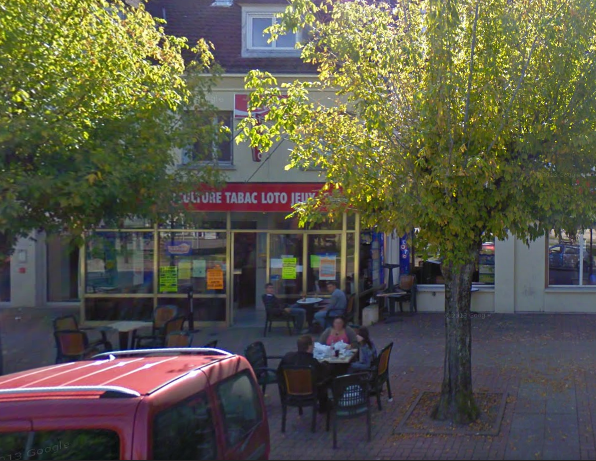
\includegraphics[scale=0.5]{BarArcis.PNG}
\end{center}

\subsection{2\ieme version}
\paragraph{}
\emph{Adams Café, Hammersmith, London :}

\paragraph{}
Le premier jour de printemps était arrivé, mais le froid était toujours au
rendez-vous. Près de la station Hammersmith, un quartier très attractif du
grand Londres, je me suis replié auprès du café Adams pour me réchauffer.

\paragraph{}
Très peu de temps après mon arrivée, une serveuse est venue vers moi pour me
proposer de boire un verre et de m’asseoir près de la grande baie vitrée du
café. Je lui répondis que je désire prendre un café avec un pancake si cela
était possible. Le café était très chic et décoré d’un bois rustique qui me
rappelait la bonne vieille époque.

\paragraph{}
Je me suis donc assis à l’endroit qu’elle m’avait proposé, je pouvais voir ces
personnes qui couraient près du « Tube Station » de la station d’Hammersmith,
très utilisé de jour comme de nuit. Dans le café, beaucoup de personne s’y
trouvait, dont un couple de personne âgé qui m’a interpellé accompagné de leur
petit fils. Ils rigolaient et semblaient heureux d’être ensemble.

\paragraph{}
Au fond du café, un homme tout seul se trouvait là, je me demandais ce qu’il
faisait et pourquoi est-ce qu’il préférait être là, plutôt que chez lui.
Réfléchissait-il à ce qu’il voulait faire dans la journée ?

\paragraph{}
Alors que j’observais les clients autour de moi, la serveuse m’interrompit en
me pausant mon café sur table en me souhaitant « Have a good lunch ».  Je la
remerciais en la saluant pour lui dire qu’elle pouvait disposer, car je n’avais
besoin de rien d’autre que d’être seul.

\paragraph{}
Pendant ce temps, un jeune couple entrèrent dans le café, avec des sacs pleins
les mains et des bagages sur le dos. À l’heure accent, j’en étais sûr, c’était
des Français. Je fus ravi qu’ils s’assoient à côté de moi, car je me suis dit
que je pouvais comprendre ce qu’ils disaient, sans même qu’ils ne sachent que
je comprenne ce qu’ils disaient.

\paragraph{}
Ces dernières racontaient leur premier ressentis de leur voyage à Londres et
semblaient véritablement conquis par l’ambiance de ces lieux.

\paragraph{}
Je déposais l’argent sur la table pour payer ce que j’avais commandé, avec ce
qu’on appelle un « tips », qui est un pourboire de 2 euros que j’ai laissé pour
cette charmante serveuse.

\paragraph{}
Avant de partir, j’ai salué les 2 Français « Have a nice day, dear countryman »
et ils ont souris, ce qui m’a fait chaud au cœur, car moi aussi j’étais heureux
de me trouver à Londres.

\subsection{3\ieme version}

\paragraph{}
\emph{18 février, Le Perrier, Châtel}

\subsubsection{Introduction}
\paragraph{}
J'ai fait mes observations dans le café de Châtel, pendant mes vacances de ski.
Ainsi, il faut garder en mémoire que l'esprit des personnes présentes dans le
café est plus centré sur les vacances et donc l'ambiance est très probablement
plus joviale que la ``normale''.

\subsubsection{Différences ethniques}
\paragraph{}
J'ai pu remarqué que les groupes entrant dans le café ne possédaient pas
beaucoup de différences ethniques. On peut donc supposer que les groupes
partant en vacances de ski (la plupart de manière familiale par suppositions)
le font la plupart du temps avec des personnes de la même ethnie.

\subsubsection{Consommations}
\paragraph{}
Parmi les boissons consommées dans différents groupes, il existe beaucoup de
similitudes entre les consommations de chaque groupe. Par exemple, un groupe
entier consommera plus des bières en général alors qu'un autre groupe
consommera des boissons plus sucrées/chaudes comme des chocolats chaud ou des
cafés.

\subsubsection{Conversations}
\paragraph{}
Pour des raisons de vie privées, je n'ai pas écouté avec précision les
conversations des personnes. Cependant avec des mots clefs, j'ai pu déduire
que les conversations tournaient en grande majorité autours du ski même
(performances, que faire ensuite). Sinon, les discussions tournaient souvent
autour des vacances.

\subsubsection{Positions}
\paragraph{}
Des comportements récurrents que j'ai pu observer étaient que la plupart du
temps les hommes dans la tranche d'âge 20-40 se mettent souvent ou presque
toujours dans les coins ou dos à un mur, laissant aux enfants des places avec
chaises du côté où d'autres personnes, étrangères, passeraient.

\subsection{4\ieme version}
\paragraph{}
\emph{Jeudi 12 février, 8h25 – Café Cours des Roches, Noisiel}

\paragraph{}
Je ne me sens pas à ma place, et en même temps je n’ai pas envie de bouger. Un
coup d’œil rapide à ma montre, huit heures vingt-cinq – trois minutes, c’est
bon, je peux attaquer mon chocolat chaud. Il n’y a rien de pire que de se
brûler la langue dans la précipitation. Mon croissant est déjà bien entamé,
mais de toute façon, je n’oserais pas le tremper dans ma tasse ; je n’ai jamais
su si c’était bien vu en public.

\paragraph{}
Il y a dix minutes, je m’installais au café, commandais chocolat, jus et
viennoiserie, avec un léger trac. L’objectif : s’asseoir et observer. Pas
facile, quand on se sent soi-même en terre inconnue : je n’ai pas l’habitude
des cafés, et eux-mêmes n’ont sans doute pas coutume de voir un étudiant de 19
ans – moins en apparence – tout seul, balayer la salle un bloc-notes à la main.

\paragraph{}
La salle est calme, peu remplie, les clients vont et viennent. La plupart ne
restent pas longtemps : nous sommes en face de la gare, et près de toutes
sortes de bureaux : trésor public, banque populaire... On vient au café des
Roches pour y déjeuner sur le pouce, en attendant ou en sortant du train. Ou
peut-être de ce cortège de bus dont les horaires ne se marient jamais à ceux du
RER. Je me félicite de ne pas être venu un jour de marché : la place et les
trottoirs y sont habituellement noirs de monde, alors je n’ose imaginer
l’atmosphère du bar.

\paragraph{}
Je remarque tout de même des profils différents du cadre de passage et du
voyageur affamé. Au comptoir, quelques habitués venus partager les dernières
nouvelles avec le patron. J’y associe sans doute trop vite le cliché habituel ;
après tout, rien ne me dit qu’il s’agit du patron, d’ailleurs je ne vois aucun
torchon sur son avant-bras. Je ne saurais nommer le contenu de leurs verres,
mais il me semble plus éthylique que mon modeste jus d’orange. Plus loin, à une
table, un jeune couple sûrement trop tôt réveillé. Difficile d’évaluer leur
profession. Aspirés par leur conversation, ils délaissent leurs boissons
chaudes. Dans quel monde vivons-nous ?

\paragraph{}
Les quelques places en terrasse – un joli mot pour désigner le trottoir – sont
délaissées, sans surprise par ce froid.  J’aperçois un groupe de trois
lycéennes s’y asseoir, puis se raviser et entrer dans le bar. On leur apporte
vite des cafés. Rien d’étonnant, le lycée Gérard de Nerval est à deux pas. Je
me surprends à penser qu’elles sont un peu jeunes pour ce genre
d’établissement, avant d’estimer que je n’avais que deux ou trois ans de plus
qu’elles. On prend souvent un café parce que c’est une boisson de grand, et on
est trahi par la quantité de sucre, de lait et de mousse saupoudrée de cacao
qu’on y instille. Ça ne manque pas ici.

\paragraph{}
J’en arrive à une conclusion : un café, c’est le lieu des grands par
excellence. Le lieu de ceux qui ont renoncé à un peu de sommeil supplémentaire
pour venir partager un verre, une tasse, un gobelet entre collègues. La société
plutôt que le rêve. Ce qui explique sans doute pourquoi je ne m’y sentais pas à
mon aise, et qu’un quart d’heure a suffi à me faire penser que ces demoiselles
devraient plutôt être en cours à huit heures et demie. Une vraie réflexion de
grand – c’est-à-dire de vieux.

\chapter{Communication Homme/Femme}
\paragraph{}
bla

\section{Hommes}
\subsection{1\ier version}
\paragraph{}
bla

\subsection{2\ieme version}
\paragraph{}
bla

\subsection{3\ieme version}
\paragraph{}
bla

\subsection{4\ieme version}
\paragraph{}
bla

\section{Femmes}
\subsection{1\ier version}
\paragraph{}
bla

\subsection{2\ieme version}
\paragraph{}
bla

\subsection{3\ieme version}
\paragraph{}
bla

\subsection{4\ieme version}
\paragraph{}
bla

\section{Mixte}
\subsection{1\ier version}
\paragraph{}
bla

\subsection{2\ieme version}
\paragraph{}
bla

\subsection{3\ieme version}
\paragraph{}
bla

\subsection{4\ieme version}
\paragraph{}
bla

\chapter{Entretiens}
\paragraph{}
bla

\subsection{1\ier version}
\paragraph{}
bla

\subsection{2\ieme version}
\paragraph{}
bla

\subsection{3\ieme version}
\paragraph{}
bla

\subsection{4\ieme version}
\paragraph{}
bla

\chapter{Enfants}
\paragraph{}
bla

\subsection{1\ier version}
\paragraph{}
bla

\subsection{2\ieme version}
\paragraph{}
bla

\subsection{3\ieme version}
\paragraph{}
bla

\subsection{4\ieme version}
\paragraph{}
bla
